\documentclass[12pt,letterpaper, titlepage]{article}
\usepackage{amssymb, amsmath, hyperref,setspace,sidenotes,todonotes}
\usepackage{color,parskip,siunitx,physics}
\DeclareMathAlphabet{\mathscr}{OT1}{pzc}{m}{it}
\usepackage{epsfig, graphicx,comment}
\usepackage{verbatim,marginfix}
%\usepackage{mparhack}
\usepackage[inner=2cm, outer=7cm, marginparsep=.5cm, marginparwidth=6cm, 
twoside=true]{geometry}
% for double partial derivatives
\title{Laser-Wakefield Electron Accelerators}
\author{Adam A. S. Green}
\begin{document}
\bibliographystyle{plain}
\maketitle

\begin{abstract}
In the late 1970's, Tajima and Dawson proposed a method of acceleration 
electron
using the large electric field gradients that plasmas are capable of 
sustaining. They showed that when a large amplitude laser pulse is sent through 
an plasma, it is capable of creating a co-propogating longitudinal plasma wave 
that is capable of having an electric field gradient of multiple Gev/cm. 

In this work, we review the state-of-the-art experimental progress being made 
in creating a fully functioning electron accelerator based on laser plasma 
acceleration (LPA) technology. We discuss how the energy in a  transverse, 
oscillitory electric field of a high intensity pulsed laser can be converted 
into an electric field gradient that can be used to accelerate electrons, and 
we will briefly review the physics of its propogation.  \end{abstract}
\tableofcontents
\section{Introduction}
\label{sec:intro}
The ability to accelerate electrons to relativistic energies ($ E > m_e c$) has 
had of the the largest impacts in modern science: leading to advances in 
particle physics, radiology, and condensed matter.
It remains one of the most systematic ways to produce collumated x-ray's.
Unfortunately, the maximum accelerating gradient able to be produced by current 
tecnology is on the scale of $\sim \SI{100}{\electronvolt.cm^{-1}}$, which, in 
order to produce relativistic
energies ($\sim \SI{.511}{\mega\electronvolt}$), requires a lot
of centimeters: CERN has a circumfrence of \SI{27}{km}. The large size needed 
has precluded the use widespread use of relativistic electrons.

In contrast, the accelerating gradient in typical LPA technology is $\sim 
\SI{1}{\giga\electronvolt.cm^{-1}}$. This then is the promise of LPA technology: 
table-top sized experiments that will allow the widespread disemmenation of 
relativistic electrons. 
\section{The Physics of Laser-Plasma-Acceleration}

\begin{marginfigure}
    \includegraphics[angle=90,width=margi

\begin{comment}
\subsection{The Need for Plasmas}
The reason that LPA has had such a resurgance is that it was only recently that 
laser technology was able to produce the electric field gradients neccesary. For 
instance, the laser used at UT-Austin in their LPA technology uses required a 
peak intensity of \SI{e18}{W.cm^{-2}} {\bf (not quite right, this is another 
group).}

It is tempting to ask why the plasma is needed at all when you have a laser 
capable of generating such high power-- why not just use the laser? In {\bf 
date} Woodward and Lauren proved that laser's cannot actually be used to 
accelerate particles, for much the same reason that boats only move up and down 
in linear ocean waves. {\bf maybe not the full story-- the ponderamotive force 
can't?}

The plasma acts as an intermediary, allowing the large electronic gradients 
present in a propogating high-intensity laser pulse to be transfered into a 
co-propogating longitudal wave. It is this longitudal wave that allows the 
electrons to be accelerated. In the section that follows, we will dicuss the 
physics behind this energy transfer in more depth.

\end{comment}

\section{The Creation and Propogation of Plasmons and Bubbles}
The full theory required to describe the current state-of-the-art LPA technology 
is
too difficult to treat analytically, so the majority of theoretical research 
currently
being done in the field uses numerics. However, the basic physics involved with 
LPA technology
can be illustrated quite simply, which can be useful to build an intuition about 
the
processes that occur. In the following sections, we will review a basic physical 
model
of the laser plasma interaction.


\subsection{Linear Regime: Cold Fluid Equations}
To first order the plasma can be treated as a set of uncoupled harmonic 
oscillators. When the high-intensity, short-pulsed laser is incident, it will 
have two main actions: the first is to accelerate\footnote{The term used to 
describe this in plasma literature is `quiver', as the time-average motion 
amounts to zero because of the oscillitory nature of the radial electric 
field.l}
electrons along the radial electric field; the second is to accelerate electrons 
along the propogation direction due to the ponderomotive force. 

The ponderomotive force is due to the gradient in electromagnetic energy along a 
pulsed laser. {\bf show gaussian picture}. It will tend to create a `bubble', as 
it expels the lighter electrons from the laser pulse, leaving the heavier ions.

In our model, the ponderomotive force will act as a driving force on the plasma,
which has a natural oscillation rate $\omega_p$.  \begin{equation}
    \label{eq:linear density oscillation}
    \qty(\pdv[2]{}{t} +\omega_p^2) \frac{\delta n_e}{n_{e0}} = c^2 \laplacian{ 
    \frac{a^2}{2}}
\end{equation}

It is this density oscillation which creates an electric field through poisson's 
equation: $\vb{k}\dotproduct\vb{E} =\delta n_e/\epsilon$. It is this
longitudinally propogating electric field that will accelerate the electrons in 
the plasma.
 
{\it still need to mention resonance}

The propogating laser packet expels electrons from its local region, which acts
as a driving force to create a co-propogating density oscillation. This creates 
in effect a cavity of ions at moves at the phase velocity of the laser packet.  
This gives rise to an electric field gradient that will be able to accelerate 
electrons.
\section{Trapping Electrons}
In order to be accelerated by the co-propogating electric field created by the
plasmon, the electrons need to be travelling at some minimum speed. In the
plasmon frame of reference, what an electron will see is, roughly, an
ion-sphere. If we confine the electrons motion to 1D, then it can exhibit
periodic motion about the centre of this sphere. 

However, for this to work, the electron needs to have some minimum energy.
Imagining a simple harmonic potential that is moving at some brisk speed $v_b >
\sqrt{2 V_\mathrm{height of well}/m} $, we can see that an electron at rest will
not be trapped: transforming to the potentials frame of reference, the electron
will have too much energy to be trapped.
\begin{marginfigure}
    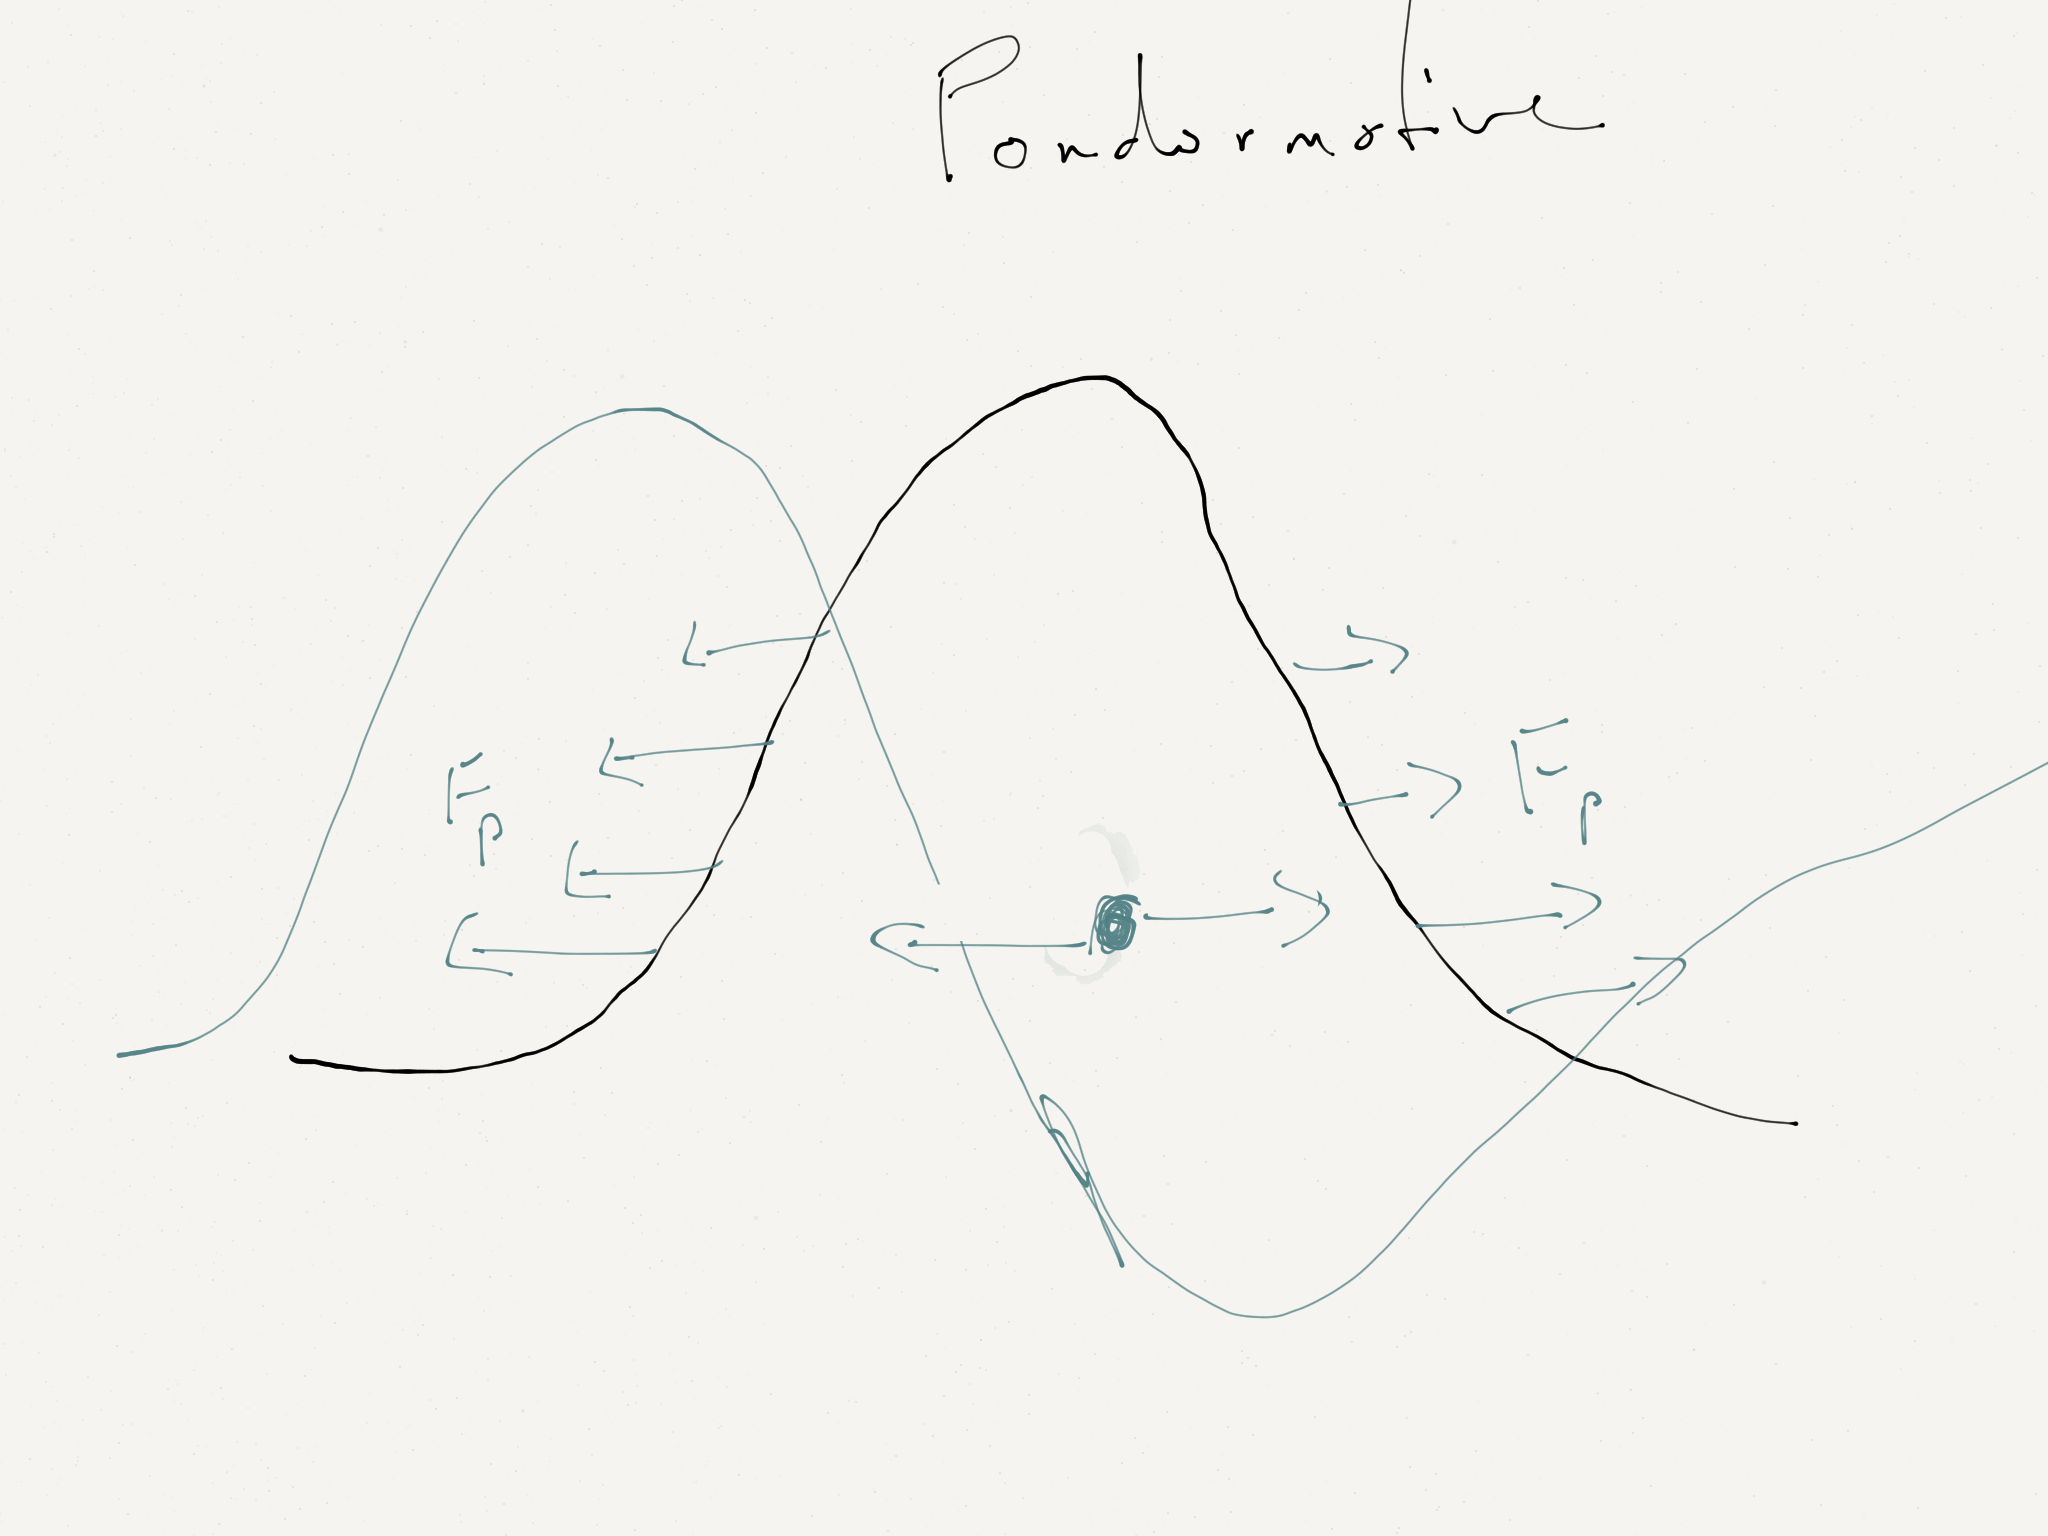
\includegraphics[width=\marginparwidth]{./Figures/pf.png}
    \caption{This shows the ponderomotive force. It will expel electrons from
        the laser
        packet region, in effect creating an ion-sphere that will create an
        accelerating force
    on a 'test' electron}
\end{marginfigure}
This is quite similar to the case we are describing: however, we now have to
consider that the electron's motion is going to be relativistic. In this case,
the minimum energy an electron needs is given by \todo{need to add citation}:
\begin{equation}
    \gamma_\mathrm{min} = \Delta \phi / (1+\beta_p) + \beta_p/(2 \Delta \phi)
\end{equation}

\todo{I'm not sure about adding this equation in. Probably take it out-- leave
    it at a general discussion and maybe show a plot of what a test electron's
trajectory would look like.}

For a very specific value of the accelerating electric field the background
electrons that make up the density flucuations will actually meet the
requirements to be trapped in this way. This gives rise to the phenomena of
wavebreaking. In contrast to the perhaps more familiar example of water-wave's
breaking, plasma wavebreaking is not a dispersion related phenomena. It is a
non-linear effect, where the accelerating field created by the density
flucuations of electrons in the plasma is strong enough to directly effect the
density flucuations themselves.

Wavebreaking is a useful phenomena for LWFA as it creates a larger field that
can give more energy to the electrons. The phenomelogical differences between a
linear plasmon and a wavebroken plasmon are show in Figure \todo{add figure}.

{\em Trapping and accleration in nonlinear plasma waves was very useful-- a
    little terse. Mainly, they just guessed the hamiltonian for the system,
    plotted traj. around the fixed points and then said that the largest energy
    gain is by largest traj in phase space. (makes sense). Then they solve for
    the minimun kinetic energy a test electron would have on the largest traj.
    This then is the minimum energy required for an electron to be caught. I'm
    still not quite sure about some of the sublties about the phase (position)
relationship to the energy.}
\subsection{Nonlinear-1D}

\subsection{Injecting Electrons into Bubbles}

\section{Experimental Set-Up and State-of-the-Art}

\section{Future Work and Outlook for the Field}

\section{Conclusion}
\end{document}

